%\documentclass[fleqn]{article}
%\documentclass[twocolumn,10pt]{article} %% original submission
%\documentclass[nocopyrightspace]{sigplanconf}

\documentclass{acm_proc_article-sp}

\usepackage{xspace,amsmath,math-cmds,
            math-envs,inference-rules,times,
            verbatim,alltt,multicol,proof,url}
\usepackage{epsfig}
\usepackage{code} 
%\setlength{\oddsidemargin}{0in}
%\setlength{\evensidemargin}{0in}
%\setlength{\textwidth}{6.5in}
%\setlength{\textheight}{8.5in}

\setlength{\hoffset}{-1in}
\setlength{\voffset}{-1in}

\setlength{\topmargin}{1in}
\setlength{\headheight}{0pt}
\setlength{\headsep}{0pt}

\setlength{\evensidemargin}{.75in}
\setlength{\oddsidemargin}{.75in}

% Text area:

\newdimen{\standardtextwidth}
\setlength{\standardtextwidth}{42pc}

\setlength{\textwidth}{\standardtextwidth}

\setlength{\topskip}{8pt}
\setlength{\columnsep}{1.5pc}
\setlength{\textheight}{54.5pc}


\author{Kenny Q. Zhu \\
	   Shanghai Jiao Tong University\\
       {\small \tt kzhu@cs.sjtu.edu.cn}
	\and Kathleen Fisher \\
	   AT\&T Labs Research\\
       {\small \tt kfisher@research.att.com}
	\and David Walker \\
	   Princeton University\\
       {\small \tt dpw@cs.princeton.edu}}
\date{}
\makeatletter
\let\@copyrightspace\relax
\makeatother

\begin{document}

\newcommand{\cut}[1]{}
\newcommand{\reminder}[1]{{\it #1 }}
\newcommand{\edcom}[1]{\textbf{{#1}}}
\newcommand{\poplversion}[1]{#1}
\newcommand{\trversion}[1]{}

\newcommand{\appref}[1]{Appendix~\ref{#1}}
\newcommand{\secref}[1]{Section~\ref{#1}}
\newcommand{\tblref}[1]{Table~\ref{#1}}
\newcommand{\figref}[1]{Figure~\ref{#1}}
\newcommand{\listingref}[1]{Listing~\ref{#1}}
%\newcommand{\pref}[1]{{page~\pageref{#1}}}

\newcommand{\eg}{{\em e.g.}}
\newcommand{\cf}{{\em cf.}}
\newcommand{\ie}{{\em i.e.}}
\newcommand{\etal}{{\em et al}}
\newcommand{\etc}{{\em etc.\/}}
\newcommand{\naive}{na\"{\i}ve}
\newcommand{\role}{r\^{o}le}
\newcommand{\forte}{{fort\'{e}\/}}
\newcommand{\appr}{\~{}}

\newcommand{\bftt}[1]{{\ttfamily\bfseries{}#1}}
\newcommand{\kw}[1]{\bftt{#1}}
\newcommand{\pads}{\textsc{pads}}
\newcommand{\padsc}{\textsc{pads/c}}
\newcommand{\padx}{\textsc{padx}}
\newcommand{\ipads}{\textsc{ipads}}
\newcommand{\ir}{\textsc{IR}}
\newcommand{\padsl}{\textsc{padsl}}
\newcommand{\padsml}{\textsc{pads/ml}}
%\newcommand{\padsd}{\textsc{pads/d}}
\newcommand{\learnpads}{{\textsc{learnpads}}}
\newcommand{\padsd}{\textsc{Gloves}}
\newcommand{\blt}{\textsc{blt}}
\newcommand{\ddc}{\textsc{ddc}}
\newcommand{\ddl}{\textsc{ddl}}
\newcommand{\C}{\textsc{C}}
\newcommand{\perl}{\textsc{Perl}}
\newcommand{\ml}{\textsc{ml}}
\newcommand{\smlnj}{\textsc{sml/nj}}
\newcommand{\ocaml}{\textsc{OCaml}\xspace}
\newcommand{\haskell}{\textsc{haskell}\xspace}
\newcommand{\ocamlbig}{\textsc{OCAML}\xspace}
\newcommand{\java}{\textsc{java}}
\newcommand{\xml}{\textsc{xml}}
\newcommand{\html}{\textsc{html}}
\newcommand{\xpath}{\textsc{xpath}}
\newcommand{\xquery}{\textsc{xquery}}
\newcommand{\datascript}{\textsc{datascript}}
\newcommand{\packettypes}{\textsc{packettypes}}
\newcommand{\erlang}{\textsc{Erlang}}
\newcommand{\camlp}{\cd{Camlp4}}
\newcommand{\ocamlnet}{\cd{Ocamlnet} \cd{2}}

\newcommand{\totalcost}[2]{\textsc{Cost}(#1,#2)}
\newcommand{\costdescription}[1]{\textsc{CT}(#1)}
\newcommand{\normcostdescription}{\textsc{NCT}}
\newcommand{\costdata}[2]{\textsc{CD}(#2 \; | \; #1)}
\newcommand{\acostdata}[2]{\textsc{ACD}(#2 \; | \; #1)}
\newcommand{\adc}[2]{\textsc{CD'}(#2 \; | \; #1)}
\newcommand{\cardt}{\textsc{Card}}
\newcommand{\costvar}[1]{\textsc{CV}(#1)}
\newcommand{\costchar}[1]{\textsc{CA}(#1)}
\newcommand{\coststring}[1]{\textsc{CS}(#1)}
\newcommand{\costint}[1]{\textsc{CI}(#1)}
\newcommand{\costparam}[1]{\textsc{CP}(#1)}
\newcommand{\costconst}[1]{\textsc{CC}(#1)}

\newcommand{\dibbler}{Sirius}
\newcommand{\ningaui}{Altair}
\newcommand{\darkstar}{Regulus}

\newcommand{\vizGems}{Arrakis}

\newcommand{\comon}{CoMon\xspace}
\newcommand{\planetlab}{PlanetLab\xspace}
\newcommand{\monall}{Monall\xspace}
%% \newcommand{}{}


%% \newcommand{\IParray}[4]{{\tt Parray} \; #1 \; \[#2, #3, #4\]}

\newcommand{\figHeight}[4]{\begin{figure}[tb]
	\centerline{
	            \epsfig{file=#1,height=#4}}
	\caption{#2}
	\label{#3}
	\end{figure}}

\newcommand{\myalt}{\ensuremath{\; | \;}}
\newcommand{\normal}[1]{\ensuremath{\bar{#1}}}
\newcommand{\relativee}[2]{\ensuremath{{\cal R}(#1 \; || \; #2)}}
\newcommand{\srelativee}[2]{\ensuremath{{\cal S}(#1 \; || \; #2)}}
\newcommand{\addh}[2]{\ensuremath{#1 \oplus #2}}

\newcommand{\irstruct}[1]{{\tt struct}\{#1\}}
\newcommand{\irunion}[1]{{\tt union}\{#1\}}
\newcommand{\irenum}[1]{{\tt enum}\{#1\}}
\newcommand{\irarray}[1]{{\tt array}\{#1\}}
\newcommand{\irarrayFW}[2]{{\tt arrayFW}\{#1\}[#2]}
\newcommand{\irswitch}[2]{{\tt switch}(#1)\{#2\}}
\newcommand{\iroption}[1]{{\tt option}\{#1\}}
\newcommand{\setof}[1]{\lsem #1 \rsem}
\newcommand{\goto}{\Rightarrow}
\newcommand{\Pvoid}{{\tt Pvoid}}
\newcommand{\Pempty}{{\tt Pempty}}
\newcommand{\sskip}{\hspace*{5mm}}
\newcommand{\shrink}{\vspace*{-4mm}}

% Semantics
\newcommand{\setalt}{{\; | \;}}
\newcommand{\denote}[1]{\lsem #1 \rsem}
\newcommand{\lsem}{{[\![}}
\newcommand{\rsem}{{]\!]}}
\newcommand{\turn}{\vdash}
\newcommand{\meta}{m}
\newcommand{\nested}{n}
\newcommand{\mytime}[1]{#1.t}
\newcommand{\myds}[1]{#1.ds}
\newcommand{\myval}[1]{#1.nest}
\newcommand{\generatedloc}{\ensuremath{\mathtt{nowhere}}}
\newcommand{\environment}{E}
\newcommand{\universe}{U}
\newcommand{\selectOne}{\ensuremath{\mathsf{earliest}}}
% core feed semantics
\newcommand{\csemantics}[3]{{\cal C}\lsem #1 \rsem_{{#2} \, {#3}}}
% feed semantics
\newcommand{\semantics}[3]{{\cal F}\lsem #1 \rsem_{{#2} \, {#3}}}
% expression semantics
\newcommand{\esemantics}[2]{{\cal E}\lsem #1 \rsem_{{#2}}}
%\newcommand{\esemantics}[2]{#2(#1)}

% Host language types
\newcommand{\ty}{\ensuremath{\tau}}
\newcommand{\basety}{\ensuremath{b}}
\newcommand{\arrow}{\rightarrow}
\newcommand{\optionty}[1]{\ensuremath{#1 \; \mathsf{option}}}
\newcommand{\listty}[1]{\ensuremath{#1 \; \mathsf{list}}}
\newcommand{\setty}[1]{\ensuremath{#1 \; \mathsf{set}}}
\newcommand{\feedty}[1]{\ensuremath{#1 \; \mathsf{feed}}}
\newcommand{\corety}[1]{\ensuremath{#1 \; \mathsf{core}}}
\newcommand{\schedulety}{\ensuremath{\mathsf{sched}}}
\newcommand{\timety}{\ensuremath{\mathsf{time}}}
\newcommand{\locty}{\ensuremath{\mathsf{loc}}}
\newcommand{\boolty}{\ensuremath{\mathsf{bool}}}
\newcommand{\unitty}{\ensuremath{\mathsf{unit}}}
\newcommand{\stringty}{\ensuremath{\mathsf{string}}}
\newcommand{\metatype}[1]{\ensuremath{\mathsf{meta}(#1)}}
\newcommand{\nestedtype}[1]{\ensuremath{\mathsf{nest}(#1)}}
\newcommand{\dsty}{\ensuremath{\mathsf{ds}}}

\newcommand{\dom}{\ensuremath{\mathsf{dom}}}
\newcommand{\ueq}[3]{\ensuremath{#1 =_{#2} #3}}
\newcommand{\fsubset}[3]{\ensuremath{#1 \subseteq_{#2} #3}}
\newcommand{\feq}[3]{\ensuremath{#1 =_{#2} #3}}

% Expressions
\newcommand{\expression}{e}
\newcommand{\constant}{c}
\newcommand{\ds}{\ensuremath{ds}}
\newcommand{\boolf}{\ensuremath{\mathtt{false}}}
\newcommand{\boolt}{\ensuremath{\mathtt{true}}}
\newcommand{\loc}{\ensuremath{\ell}}
\newcommand{\feed}{\ensuremath{F}}
\newcommand{\corefeed}{\ensuremath{C}}
\newcommand{\generalvar}{\ensuremath{x}}
\newcommand{\feedvar}{\ensuremath{x}}
\newcommand{\itemvar}{\ensuremath{x}}
\newcommand{\data}{\ensuremath{v}}
\newcommand{\atime}{\ensuremath{t}}
\newcommand{\astring}{\ensuremath{w}}
\newcommand{\unit}{\ensuremath{()}}
\newcommand{\schedule}{\ensuremath{s}}
\newcommand{\parser}{\ensuremath{p}}
\newcommand{\none}{\ensuremath{\mathtt{None}}}
\newcommand{\some}[1]{\ensuremath{\mathtt{Some}\; #1}}
\newcommand{\inl}[1]{\ensuremath{\mathtt{inl}\; #1}}
\newcommand{\inr}[1]{\ensuremath{\mathtt{inr}\; #1}}
\newcommand{\casedata}[2]{{\tt switch}(#1)\{#2\}}
%\newcommand{\nillist}{\ensuremath{\mathtt{nil}}}
\newcommand{\nillist}{\ensuremath{[\,]}}
%\newcommand{\conslist}[2]{\ensuremath{\mathtt{cons} (#1,#2)}}
\newcommand{\conslist}[2]{\ensuremath{[#1,\ldots,#2]}}
\newcommand{\nilstream}{\ensuremath{\mathtt{done}}}
\newcommand{\consstream}[2]{\ensuremath{\mathtt{next} (#1,#2)}}


% Feeds
\newcommand{\comprehensionfeed}[3]{\ensuremath{\mathtt{\{|} #1 \; \mathtt{|}\; #2 \leftarrow #3 \mathtt{|\}}}}
\newcommand{\computed}[3]{\ensuremath{\mathtt{[} #1 \; \mathtt{|}\; #2 \in #3 \mathtt{]}}}
\newcommand{\letfeed}[3]{\ensuremath{\mathtt{let}\; #1 \; \mathtt{=}\; #2 \; \mathtt{in} \; #3}}
\newcommand{\allfeed}[5]{
  \ensuremath{
    \mathtt{all \{ format=} #1; 
    \mathtt{src=} #2;
    \mathtt{sched=} #3;
    \mathtt{pp=} #4;
    \mathtt{win=} #5;
  \mathtt{\}}}}
\newcommand{\existsfeed}[5]{
  \ensuremath{
    \mathtt{any \{ format=} #1; 
    \mathtt{src=} #2;
    \mathtt{sched=} #3;
    \mathtt{pp=} #4;
    \mathtt{win=} #5;
  \mathtt{\}}}}
\newcommand{\filterfeed}[2]{
  \ensuremath{
    \mathtt{filter} \; #1 \; \mathtt{with}\; #2}}
\newcommand{\remapfeed}[2]{
  \ensuremath{
    \mathtt{redirect} \; #1 \; \mathtt{with}\; #2}}
\newcommand{\ppfeed}[2]{
  \ensuremath{
    \mathtt{pp} \; #1 \; \mathtt{with}\; #2}}
\newcommand{\foreachupdate}[3]{
  \ensuremath{
    \mathtt{foreach{*}{*}}\; #1 \;
    \mathtt{in}\; #2 \;
    \mathtt{update}\; #3}}
\newcommand{\foreachcreate}[3]{
  \ensuremath{
    \mathtt{foreach*}\; #1 \;
    \mathtt{in}\; #2 \;
    \mathtt{create}\; #3}}
\newcommand{\remap}[2]{\ensuremath{\mathtt{redirect}\; #1 \; \mathtt{with} \; #2}}
\newcommand{\stutterfeed}[2]{\ensuremath{\mathtt{stutter}\; #1 \; \mathtt{on} \; #2}}
\newcommand{\refeed}[2]{\ensuremath{\mathtt{reschedule}\; #1 \; \mathtt{to} \; #2}}
\newcommand{\emptyfeed}{\ensuremath{\emptyset}}
\newcommand{\onefeed}[2]{\ensuremath{\mathtt{One}}(#1,#2)}
\newcommand{\sfeed}[1]{\ensuremath{\mathtt{SchedF}}(#1)}
\newcommand{\lfeed}[1]{\ensuremath{\mathtt{ListF}}(#1)}
\newcommand{\unionfeed}{\ensuremath{\cup}}
\newcommand{\sumfeed}{\ensuremath{+}}
\newcommand{\spairfeed}{\; \ensuremath{\mathtt{\&} \; }}
\newcommand{\allpairfeed}{\; \ensuremath{{*}{*}} \; }

\newcommand{\Time}{\ensuremath{\mathtt{Time}}}
\newcommand{\Set}{\ensuremath{\mathtt{Set}}}

% this is used for the translations equal
\newcommand{\transeq}{\stackrel{def}{=} }
\newcommand{\ai}{{\tt wl}}



% BNF
%\newcommand{\bnfalt}{\ |\ }


%\twocolumn[\maketitle]

\title{Incremental Learning of System Log Formats}
%\subtitle{[Extended Abstract]}

\author{
\numberofauthors{3}
\alignauthor
  Kenny Q. Zhu \\
  \affaddr{Shanghai Jiao Tong University} \\
  \email{kzhu@cs.sjtu.edu.cn}
\alignauthor
  Kathleen Fisher \\
  \affaddr{AT\&T Labs Research} \\
  \email{kfisher@research.att.com}
\alignauthor
  David Walker \\
  \affaddr{Princeton University} \\
  \email{dpw@cs.princeton.edu}
}

\maketitle

Many applications use the file system as a simple persistent data
store.  Although this approach is expedient, imposing almost no
overhead, it is not robust because in general, the overall correctness
of the application will depend on the collection of files,
directories, and symbolic links in the file system having some precise
hierarchical organization and metadata such as file ownership,
permissions, and timestamps but current programming languages do not
provide support for documenting assumptions about the file system. In
addition, actually loading the data from the disk requires writing a
lot of distracting boilerplate code.

This paper describes \forest{}, a new domain-specific language for
describing directory structures embedded in \haskell{}. \forest{}
descriptions use a type-based metaphor to specify portions of the file
system in a simple, declarative manner.  \forest{} makes it easy to
connect data on the disk to an isomorphic representation in memory
that can be manipulated by programmers as if it were any other
strongly-typed data structure in their program.  \forest{} also
generates metadata that can be used to verify that a given portion of
the file system conforms to its specification.  It greatly lowers the
divide between on-disk and in-memory representations of data.

We present our design for \forest{} and describe an implementation of
a full working prototype in \haskell{}. From a single compact
description, the \forest{} implementation generates a useful
collection of \haskell{} types and functions for manipulating,
checking, and analyzing file system data.   In addition, \forest{}
generates type class definitions that make it possible to
exploit powerful
generic programming paradigms that
allow third-party developers to build tools for querying,
visualizing, and debugging on-disk data in a generic way. We
present examples illustrating the use of \forest{} on a number of
real-world directory structures and programming tasks, including
drop-in replacements for a number of standard shell tools. Finally, we
formalize the core elements of the language as a simple calculus based
on classical tree logics.

\category{D.4.9}{Operating Systems}{Systems Programs and Utilities}
\category{D.3.4}{Programming Languages}{Processors}

\terms
Languages, Algorithms

\keywords
Grammar induction, analysis of system logs, domain-specific languages, parsing,
tool generation, ad hoc data, PADS

\section{Introduction}
\label{sec:intro}

{\em Data description languages} are a class of domain specific
languages for specifying {\em ad hoc data formats}, from billing 
records to TCP packets to scientific data sets to server logs.  Examples 
of such languages include 
\bro~\cite{paxson:bro}, \datascript{}~\cite{gpce02}, \demeter~\cite{lieberherr+:class-dictionaries},
\packettypes{}~\cite{sigcomm00}, \padsc{}~\cite{fisher+:pads}, 
\padsml{}~\cite{mandelbaum+:padsml}  and
\xsugar~\cite{xsugar2005}, among others.  All of these languages
generate parsers from data descriptions.  In addition, and unlike
conventional parsing tools such as Lex and Yacc, many also automatically
generate auxiliary tools ranging from printers to \xml{} converters to
visitor libraries to visualization and editor tools.

In previous work, we developed the {\em Data Description Calculus}
(\ddcold{}), a calculus of simple, orthogonal type constructors,
designed to capture the core features of many existing type-based data
description languages~\cite{fisher+:next700ddl,fisher+:ddcjournal}.
This calculus had a multi-part denotational semantics that interpreted
the type constructors as (1) parsers the transform external bit
strings into internal data representations and {\em parse descriptors}
(representations of parser errors), (2) types for the data
representations and parse descriptors, and (3) types for the parsers
as a whole.  We proved that this multi-part semantics was coherent in
the sense that the generated parsers always have the expected types
and generate representations that satisfy an important {\em
canonical forms} lemma.

The \ddcold{} has been very useful already, helping us debug and
improve several aspects of \padsc{}~\cite{fisher+:pads}, and serving
as a guide for the design of \padsml{}~\cite{mandelbaum+:padsml}.
However, this initial work on the \ddcold{} told only a fraction of the
semantic story concerning data description languages.  As mentioned
above, many of these languages not only provide parsers, but
also other tools.  Amongst the most common auxiliary tools
are printers, as reliable communication between programs, either through
the file system or over the Web, depends upon both input (parsing) 
and output (printing).

In this work, we begin to address the limitations of
\ddcold{} by specifying a printing semantics for the
various features of the calculus.  We also
prove a collection of theorems for the new semantics that serve as
duals to our theorems concerning parsing.  This new printing semantics
has many of the same practical benefits as our older parsing 
semantics: We can
use it as a check against the correctness of our printer
implementations and as a guide for the
implementation of future data description languages.  


% First, we extend \ddcold{} with
% abstractions over types, which provides a basis for specifying the
% semantics of \padsml{}. In the process, we also improve upon the
% \ddcold{} theory by making a couple of subtle changes. For example, we
% are able to eliminate the complicated ``contractiveness'' constraint
% from our earlier work. Second, .

% The main practical benefit of the calculus has been as a guide for our
% implementation. Before working through the formal semantics, we
% struggled to disentangle the invariants related to polymorphism. After
% we had defined the calculus, we were able to implement type
% abstractions as \ocaml{} functors in approximately a week.  Our new
% printing semantics was also very important for helping us define and
% check the correctness of our printer implementation.  We hope the
% calculus will serve as a guide for implementations of \pads{} in
% other host languages.  

% In summary, this work makes the following key contributions:
% \begin{itemize}
% \item We simultaneously specify both a parsing and a printing semantics
%   for the \ddc{}, a calculus of polymorphic, dependent types.
% \item We prove that \ddc{} parsers and printers are type safe
%   and well-behaved as defined by a canonical forms theorem.
% \end{itemize}

In this extended abstract, we give an brief overview of the calculus,
it's dual semantics and their properties.  A companion technical
report contains a complete formal
specification~\cite{fisher+:popl-sub-long}.  In comparison to our
previous work on the \ddcold{} at POPL 06~\cite{mandelbaum+:padsml},
the calculus we present here has been streamlined in several subtle,
but useful ways.  It has also been improved through the addition of
polymorphic types.  We call this new polymorphic variant
\ddc{}.  These improvements and extensions, together with
proofs, appear in Mandelbaum's thesis~\cite{mandelbaum:thesis} and in
a recently submitted journal article~\cite{fisher+:ddcjournal}.
This abstract reviews the \ddc{} and extends all the previous 
work with a printing semantics and appropriate theorems.
To be more specific,
sections~\ref{sec:ddc-syntax} through \ref{sec:ddc-sem} present the
extended \ddc{} calculus, focusing on the semantics of polymorphic
types for parsing and the key elements of the printing semantics.
Then, \secref{sec:meta-theory} shows that both parsers and
printers in the \ddc{} are type correct and furthermore that parsers
produce pairs of parsed data and parse descriptors in {\em canonical
  form}, and that printers, given data in canonical form, print
successfully. We briefly discuss related work in \secref{sec:related}, and
conclude in \secref{sec:conc}.

%%% Local Variables: 
%%% mode: latex
%%% TeX-master: "paper"
%%% End: 


Our format inference algorithm is implemented as a series of phases that
generate and transform an internal format description language we
refer to simply as the \ir.  The \ir{} is very similar to
the \ipads{} language we developed and formalized in previous 
work~\cite{fisher+:popl06}.  Apart from syntax, the main differences 
are that the \ir{} omits recursion and function declarations; the former
being beyond the scope of our current inference techniques and the 
latter being unnecessary during the course of the inference algorithm.  
%In addition, for convenience during inference, the scope of dependent 
%variable binding is slightly different, as will be explained below.

\begin {figure}
{\small
\begin {tabular}{llll}
%\multicolumn{4}{l}{
%\begin {tabular}{llll}
$c$ & ::= & $a$ \myalt $i$ \myalt $s$ & (constants)\\
$x$ & & & (variables) \\
$p$ & :: = & $c$ \myalt $x$ & (parameters) \\
\\
\end{tabular}

\begin {tabular}{ll}
\multicolumn{2}{l}{Base types $b$  ::=} \\
\hspace{5pt} \cd{Pint} &                  (generic, unrefined integer) \\
\myalt \cd{PintRanged} &             (integer with min/max values) \\
\myalt \cd{Pint32} &                 (32-bit integer) \\
\myalt \cd{Pint64} &                (64-bit integer) \\
\myalt \cd{PintConst} &              (constant integer) \\
\myalt \cd{Pfloat} &                (floating point number) \\
\myalt \cd{Palpha} &                (alpha-numeric string) \\
\myalt \cd{Pstring} &               (string; terminating character) \\
\myalt \cd{PstringFW} &             (string; fixed width) \\
\myalt \cd{PstringConst} &          (constant string) \\
\myalt \cd{Pother} &                (punctuation character) \\
\myalt \cd{ComplexB} &              (complex base type defined by regexp; \\
                                     & \hspace{5pt} \eg{} date, time, \etc{}) \\
\myalt \cd{Pvoid} &                 (parses no characters; fails immediately) \\
\myalt \cd{Pempty} &                (parses no characters; succeeds immediately) \\
\\
\end {tabular}

\begin {tabular}{ll}
\multicolumn{2}{l}{Types $T$ ::= } \\ 
\hspace{5pt} $b$($p_1$,...,$p_k$)&          (parameterized base type) \\
\myalt  $x$:$b$($p_1$,...,$p_k$) &         (parameterized base type; \\
                                & \hspace{5pt} underlying value named x)    \\  
\myalt  \cd{struct} \{$T_1$; ... $T_k$;\}&   (fixed sequence of items) \\
\myalt  \cd{array} \{$T$;\} &            (array with unbounded repetitions) \\
\myalt  \cd{arrayFW} \{$T$;\}[$p$]&        (array; fixed length)  \\
\myalt  \cd{arrayST} \{$T$;\}[sep,term]& (array; separator and terminator) \\
\myalt  \cd{union} \{$T_1$; ... $T_k$;\} &   (alternatives) \\
\myalt  \cd{enum} \{$c_1$; ... $c_k$;\} &    (enumeration of constants) \\
\myalt  $x$:\cd{enum} \{$c_1$; ... $c_k$;\} &         (parameterized enum type; \\
                                & \hspace{5pt} underlying value named x)    \\  
\myalt  \cd{option} \{$T$;\} &           (type T or nothing) \\
\myalt  \cd{switch} $x$ \cd{of} \\
\hspace{6pt} \{$c_1$ \cd{=>} $T_1$; $\ldots$ $c_k$ \cd{=>} $T_k$;\} & (dependent choice) \\
\\
\end {tabular}

\begin {tabular}{ll}
\multicolumn{2}{l}{Representations of parsed data $d$  ::= } \\
\hspace{5pt} $c$ &        (constant) \\
\myalt  in$_i$($d$) &    (injection into the $i^{th}$ alternative of a union) \\
\myalt  ($d_1$,$\ldots$,$d_k$) &  (sequence of data items) \\
\end{tabular}
}
\caption {Selected elements of the \ir{}.} \shrink
\label{fig:ir}
\end{figure}


\begin{figure*}
Crashreporter.log:
{\small \begin{verbatim}
Sat Jun 24 06:38:46 2006 crashdump[2164]: Started writing crash report to: /Logs/Crash/Exit/ pro.crash.log
- crashreporterd[120]: mach_msg() reply failed: (ipc/send) invalid destination port
\end{verbatim}
}

Sirius AT\&T Phone Provisioning Data:
{\small \begin{verbatim}
8152272|8152272|1|6505551212|6505551212|0|0||no_ii152272|EKRS_6|0|FRED1|DUO|10|1000295291
8152261|8152261|1|0|0|0|0||no_ii752261|EKRS_1|0|kfeosf2|DUO|EKRS_6|1001390400|EKRS_OS_10|1001476801
\end{verbatim}
}

% ASL.log:
% {\small  \begin{verbatim}
% [Time 2006.11.25 16:47:18 UTC] [Facility user] [Sender E_e,] [PID 131] \
%   [Message sleep canceled time is: Sat Nov 25 08:47:18 2006;;] [Level 1] [UID -2] [GID -2] [Host Babylon]
% [Time 2006.11.25 16:51:23 UTC] [Facility install] [Sender Software Update] [PID 1879] \
%   [Message System requesting sleep.] [Level 5] [UID -2] [GID -2] [Host Babylon]
% \end{verbatim}
% }

% Apache Web Server Logs:
% {\small \begin{verbatim}
% 68.142.249.179 - - [13/Dec/2005:19:41:48 -0800] "GET /bridge-loan.html HTTP/1.0" 404 298 "-" \
%   "Mozilla/5.0 (compatible; Yahoo! Slurp; http://help.yahoo.com/help/us/ysearch/slurp)"
% 69.227.61.241 - - [13/Dec/2005:19:44:42 -0800] "GET / HTTP/1.1" 403 4251 "-" \
%   "Mozilla/5.0 (Windows; U; Windows NT 5.1; en-US; rv:1.8) Gecko/20051111 Firefox/1.5"
% \end{verbatim}
% }

\caption {Example ad hoc data sources.} \shrink
\label{fig:example}
\end{figure*}



% The end goal of this project depends
% crucially on having both interpretations of these types.  The first
% interpretation is necessary to generate a
% parser and printer for the format.  The second interpretation 
% is necessary in order to define and
% implement useful generic algorithms, such as the xml translator, that
% walk over parsed data in memory.  

\subsection{The Language}

Like all languages in the \pads{} family, the \ir{} is a collection of
type definitions.  These ``types'' define both the external syntax of
data formatted on disk and the shape of the internal representations
that result from parsing.  We rely upon both of these aspects of type
definitions to generate stand-alone tools automatically.
%-- the first is necessary for generating parsers and printers; the
%second is necessary for implementing generic algorithms such as the 
%\xml{} translator.  In the following discussion, we focus on
%explaining the first interpretation, counting on the reader's intuition 
%for the second. 
Figure~\ref{fig:ir} summarizes the syntax of the \ir{} and of the
generated internal representations. 

The building blocks of any \ir{} data description are the base types $b$,
which may be parameterized by some number of arguments $p$.  Arguments
may either be constants $c$, which include characters $a$, integers
$i$ and strings $s$, or variables $x$ bound earlier in the description.
These base types include a wide range of different sorts of
integers and strings.  In its initial phases, the inference algorithm
uses general integer \cd{Pint}, alphanumeric string \cd{Palpha}
and punctuation character \cd{Pother(}$a$\cd{)} types.  In later phases,
these coarse-grained base types are analyzed, merged and refined, producing
integers with ranges \cd{PintRanged(min,max)},
integers with known size \cd{Pint32} or \cd{Pint64}, constant integers
(\cd{PintConst(}$i$\cd{)} for some integer $i$), or floating-point
numbers \cd{Pfloat}.  Likewise, later stages of our algorithm transform
alphanumeric strings into arbitrary strings with terminating characters
(\cd{Pstring(}$a$\cd{)} where $a$ terminates the string), fixed width
strings (\cd{PstringFW(}$i$\cd{)} where $i$ is the length of the string) 
or string constants \cd{PstringConst(}$s$\cd{)}.  For brevity in
our descriptions, we normally just write the constant string $s$
inline in a description instead of \cd{PstringConst(}$s$\cd{)}.

In addition to these simple base types, the \ir{} includes a
collection of higher-level base types commonly found in ad hoc data,
specified generally in Figure~\ref{fig:ir} as \cd{ComplexB}.  For
example, we have implemented base types for IP addresses, email
addresses, URLs, XML tags, dates, times and a variety of
others. Finally, the types \cd{Pvoid} and \cd{Pempty} are two special
base types that are introduced at various points in the inference
process.  The first fails immediately; the second succeeds
immediately.  Neither consumes any characters while parsing.

Complex descriptions are built from simpler ones using a variety of
type constructors.  Type constructors include
basic struct types \cd{struct}\{$T_1$; ... $T_k$;\}, which indicate a
data source
should contain a sequence of items matching $T_1$, ..., $T_k$,
basic array types \cd{array} $T$, which indicate a data source should contain
a sequence of items of arbitrary length, each matching $T$,
and union types \cd{union} \{$T_1$; ... $T_k$;\}, which indicate a
data source
should match one of $T_1$, ..., $T_k$.  Once again, initial phases
of the inference algorithm restrict themselves to one of these three
sorts of type constructors.  However, later phases of the algorithm
refine, merge and process these simple types in a variety of ways.
For example, unions may be transformed into 
enumerations of constants
\cd{enum} \{$c_1$; ... $c_k$;\}
or options \cd{option} \{$T$;\}.  In
addition, later phases of the algorithm 
bind variables to the results of parsing 
base types and enums.  For example, $x$:$b$($p_1$,...,$p_k$) expresses the fact that
variable $x$ is bound to the value parsed by base type
$b$($p_1$,...,$p_k$).  These variables express dependencies between 
different parts
of a description.\footnote{For the purposes of inference, 
every bound variable is assumed to be distinct
from every other that appears in a description.  Roughly speaking,
the scope of such variables
extends as far as possible to the right through the description.
Understanding the fine details of the semantics is not important
for understanding the central material in this paper.}  
For example, the length of a string \cd{PstringFW}($p$)
or an array \cd{ParrayFW}($p$) may depend upon either a constant or
a variable and likewise for any other parameterized base type.  In
addition, unions may be refined into dependent switch statements
\cd{switch} $x$ \cd{of} \{$c_1$ \cd{=>} $T_1$; $\ldots$ $c_k$ \cd{=>} $T_k$;\}, where the
data is described by $T_1$, ..., or $T_k$ depending on the value
associated with $x$, be it $c_1$, ..., or $c_k$.

The result of parsing according to a description is an internal
representation of the data. We let metavariable $d$ range over such 
data representations.  For the purposes of this paper, a data 
representation may be a constant $c$, an injection into the $i^{th}$
variant of a union \cd{in}$_i(d)$, or a sequence of data representations
$(d_1,\ldots,d_k)$.  The injections are used as the representations of
any sort of union type, be it a union, an enumeration, an option or a switch.
The sequences are used as the representations of any sort of sequence
type, whether it be a struct or one of the array variants.

\subsection{Running Examples}

Figure~\ref{fig:example} presents tiny fragments of two
different ad hoc data files on which we have trained our inference algorithm.
The first, Crashreporter.log, is a Macintosh
system file that records information concerning process crashes.\footnote{For
expository purposes we have made a minor alteration to the Crashreporter.log
format to allow us to explain more concepts with a single example.
The evaluation section reports results on both the  
completely unmodified Crashreporter.log and the modified version.} 
The second, which we call Sirius, is an internal AT\&T format used to
record phone call provisioning information. 
%The third format is
%a generic system logging file called ASL.log, again taken from a
%Macintosh.
We use the Crashreporter.log data source as our main example throughout the
paper; periodically we refer to the Sirius data source to illustrate 
particular aspects of the inference algorithm.  
%We report on our experience
%with many more examples in the evaluation section of the paper.

\begin{figure}[t]
\begin{small}
\begin{verbatim}
dumpreport =
  union {
    struct {
      "Started writing crash report to: "; 
      file:Ppath;
    };
    struct {
      "Finished writing crash report to: "; 
      file:Ppath;
    };
    struct {
      "Unable to determine task_t for pid: "; 
      pid:Pint32; " name: Exited process";
    };
    struct {
      "Failed to re-launch "; 
      file:Ppath; " - "; message:Pstring('\n')
    };
  };

reporterreport =
  struct {
    function: Ppath; " reply failed: ");
    failuremsg: Pstring_('\n'); 
  };

dateoption = 
  union {
    "- ";
    struct {
      day:    PDate;  " ";
      time:   PTime;  " ";
      year:   Pint32; " ";
    };
  };

source =
  arrayST {
    struct {
      date:   dateoption;
      kind:   enum {"crashdump"; 
                    "crashreporterd";}; "[";
      dumpid: Pint32; "]: ";
      report: 
        switch kind of {
          "crashdump"      => dumpreport
          "crashreporterd" => reporterreport
    };
  }['\n',EOF];
\end{verbatim}
\end{small}
\caption{Hand-written \ir{} Crashreporter.log description.}
\label{fig:crashreporter:ir}
\end{figure}


Figure \ref{fig:crashreporter:ir} presents a hand-written description
of the Crashreporter.log file in the \ir{} syntax.  This
description is most easily read from the bottom, starting
with the definition of the \cd{source} type.  This definition specifies that
the data source is an
array of structs separated by newline characters and
terminated by the end of file marker.  In other words,
the data source is a sequence of lines, with the struct
in question appearing on each line.  
The struct itself indicates each line is a sequence of
\cd{dateoption}, \cd{kind}, \cd{dumpid} and \cd{report} fields.  
The description also specifies that the delimiter \cd{"["} 
appears between the \cd{kind} and \cd{dumpid} fields, and the
delimiter \cd{"]: "} appears between the \cd{dumpid} and 
\cd{report} fields.

%% The reader can
%% \cd{dateoption} type (appearing above the definition of \cd{source})
%% is defined as either a dash or a structure containing a \cd{PDate}
%% (one of the complex base types our system uses), a \cd{PTime} (another
%% complex base type) and an integer year.  In between each of the three
%% fields in the \cd{dateoption} struct is a space character (written
%% \cd{" "}).

Most of the variable names associated with fields (\eg{}
\cd{date}, \cd{dumpid}, \etc{}) merely serve as documentation for the reader.
However, the \cd{kind} field is different -- it is used later in the 
description and hence illustrates a {\em dependency}.  
To be specific, the form of the
\cd{report} field depends upon the contents of the \cd{kind}
field.  If its value is \cd{"crashdump"}, then the \cd{report} is
a \cd{dumpReport} type, while if the \cd{kind} field is \cd{"crashreporterd"},
the \cd{report} is a \cd{reporterReport} type.  

Figure~\ref{fig:crashreporter:ir} contains three other definitions
aside from \cd{source}.  These definitions specify the
structure of the  \cd{dumpReport}, \cd{reporterReport} and \cd{dateOption}
types.

%% specify the component parts
%% The definition of \cd{reporterreport} is relatively simple -- it is
%% a structure containing a file path 
%% (\cd{Ppath} is one of the complex base types our system uses) and 
%% a message following 
%% \cd{" reply failed: "}.  A \cd{crashdump} message is more complicated --
%% it is a union of several different possible message formats. Finally, a
%% \cd{dateoption} type 
%% is defined as either a dash or a structure containing a \cd{PDate}, 
%% a \cd{PTime} and an integer year. 




%%% Local Variables: 
%%% mode: latex
%%% TeX-master: "paper"
%%% End: 


\section{Main Algorithm}\label{sec:algo}
The \learnpads{} algorithm in \secref{sec:review}  produces good results for the small
log files that we have experimented with, but it has two limitations:
performance and adaptability.  In terms of performance, the algorithm
requires space quadratic in the input file size to perform the data
dependency analysis, so it cannot be used on data sources larger than the
square root of the size of usable memory. In terms of adaptability, the
algorithm only learns a description from a fixed amount of data.
If the data changes over time,
the algorithm cannot modify the existing description; 
it must start from scratch. This prevents the user from adapting
descriptions to manage evolving data sources.

To address these problems, we extended \learnpads{} to work
incrementally.  
\figref{fig:overview} illustrates the overall process.
Given a candidate description \cd{D}, the new algorithm uses \cd{D} to parse
the records in the data source.  
It discards records that parse successfully, since these records are
already covered by \cd{D}, but it collects records that fail to parse.
Specifically, if a portion of a record fails to parse,
that failure will be detected at a particular node in \cd{D}.
These failed portions are collected
in an aggregation data structure \cd{A} that mirrors the the structure
of \cd{D}. When the algorithm accumulates $M$ such records, where $M$ is a
parameter of the algorithm, it transforms \cd{D} to accommodate the places 
where differences were found (\ie, by introducing options where a piece of
data was missing or unions where a new type of data was discovered).
It then uses the original \learnpads{} algorithm to infer descriptions
for the aggregated portions of bad data, and merge these new
sub-descriptions into the transformed description to produce a new,
refined description \cd{D'}. This refined
description subsumes \cd{D} and describes the $M$
new records.  In addition, the algorithm attempts to preserve as much
of the structure of \cd{D} as possible, so users supplying initial
descriptions can recognize the resulting descriptions. 
The algorithm then makes \cd{D'}
the new candidate description and repeats the process until it
has consumed all the input data. We call the main loop in 
\figref{fig:overview} the {\em incremental learning step}.
The initial description \cd{D} can either be supplied by a user or it
can be inferred automatically by applying the original algorithm to
$N$ records selected from the data source, where $N$ is another
parameter.  
%Currently, the system selects a mix of $N/3$ consecutive lines
%taken from the beginning, middle, and end of the data source. 

\cut{%%%%%%%%%%%%%%%%
Intuitively, the incremental learning step works by attempting to
parse each of the $M$ records according to the current description
\cd{D}.  It discards the portions of each record that parse correctly.
If a portion fails to parse, that failure will be detected at a
particular node in the description \cd{D}. It collects these failed
portions in an aggregation data structure \cd{A} that mirrors the
structure of \cd{D}.  After thus aggregating all the failures in the $M$
records, the algorithm transforms \cd{D} to accommodate the places where
differences were found (\ie, by introducing options where a piece of
data was missing or unions where a new type of data was discovered).
It then uses the original \learnpads{} algorithm to infer descriptions
for the aggregated portions of bad data. 
}%%%%%%%%%% end of cut

In the following, we present the algorithm in more detail.

\cut{
Intuitively, the incremental learning algorithm takes an initial
description as input, divides the new data into manageable
chunks, and iteratively merges descriptions of these chunks into the
current description.
\figref{fig:overview} illustrates a high level schematic of this
algorithm. A large or streaming data source is input 
to the system in batches. Each batch of data contains $M$ 
records, where $M$ is a parameter of the framework.
%%The state of the system is determined by the current data
%%description which is subject to change as new data streams into the system. 
The initial description
can be supplied by user, or learned from the first batch of the input
data. At each iteration, the system generates a filter program from
the current data description.  This program parses the incoming batch of data
into an aggregated data structure similar to the parse tree of the description.
In this process, the filter program collects ``bad data'' which does not
conform to the current description. The system then invokes the original
\learnpads{} algorithm to learn ``sub-descriptions'' from the bad data, and
merges these sub-descriptions into the current data description to produce
a new description for the next iteration. 
}
\begin{figure}[t]
\centering
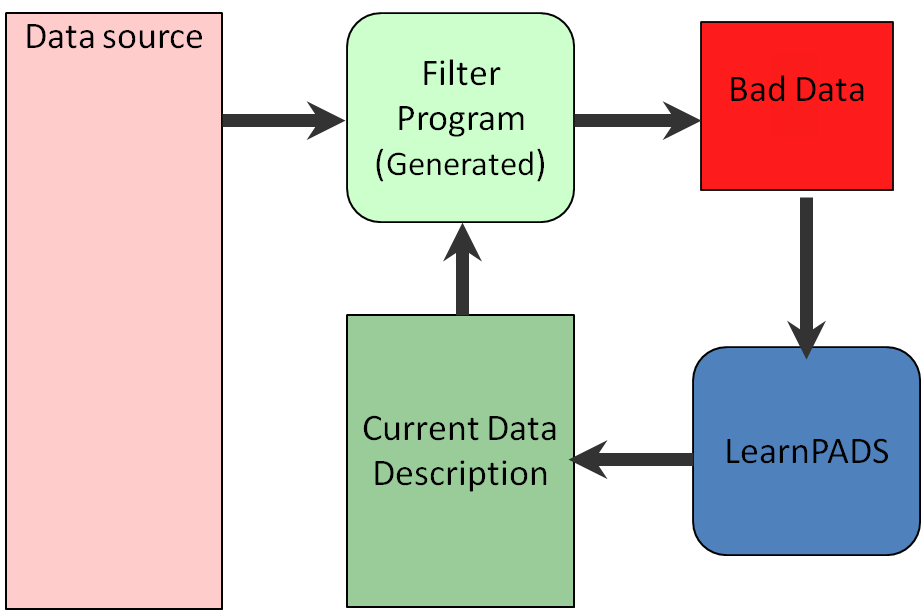
\includegraphics[width=0.8\columnwidth]{overview}
%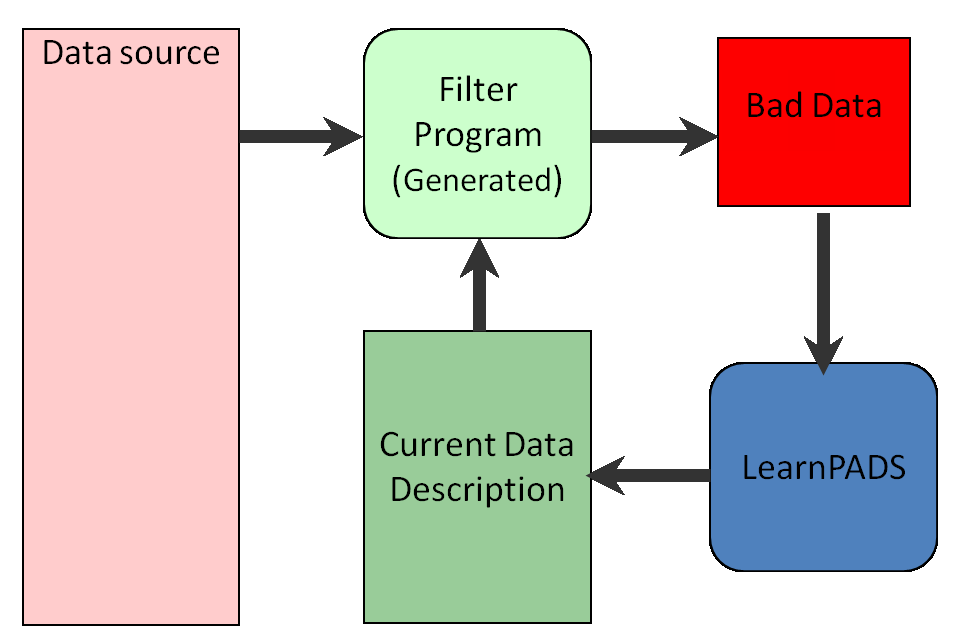
\epsfig{file=overview.eps,width=0.9\columnwidth}
\caption{An Overview of the Incremental Learning Framework}
\label{fig:overview}
\vskip -2ex
\end{figure}

%To address these problems, 
%we extended \learnpads{} to work incrementally.  
%Given a candidate description \cd{D}, the new algorithm uses \cd{D} to parse
%the records in the data source.  
%It discards records that parse successfully, since these records are
%already covered by \cd{D}, but it collects records that fail to parse.
%When the algorithm accumulates $M$ such records, where $M$ is a
%parameter of the algorithm, it invokes the incremental learning step,
%described below, to produce a refined description \cd{D'}.  This refined
%description subsumes \cd{D} and describes the $M$
%new records.  In addition, the algorithm attempts to preserve as much
%of the structure of \cd{D} as possible, so users supplying initial
%descriptions can recognize the resulting descriptions. 
%The algorithm then takes \cd{D'}
%to be the new candidate description and repeats the process until it
%has consumed all the input data.
%The initial description \cd{D} can either be supplied by a user or it
%can be inferred automatically by applying the original algorithm to
%$N$ records selected from the data source, where $N$ is another
%parameter.  
%Currently, the system selects a mix of $N/3$ consecutive lines
%taken from the beginning, middle, and end of the data source. 

\subsection{Preliminaries}

\begin{figure}[t]
{\small 
\begin{code}
\kw{Basic notation}:
c            (a string character)	
s1.s2        (concatenation of strings)
first(s)     (first character of s)
prefix(s)    (set of prefixes of s) 
sprefix(s)   (set of strict prefixes of s)
len(s)       (length of s)
\end{code}
\begin{code}
\kw{Descriptions}:
Base ::= Pint | PstringME(re) | PstringFW(e)
\end{code}
\begin{code}
D ::=   
  Base               (Base token)
| Sync s             (Synchronizing token) 
| Pair (x:D1, D2)    (Pair with dependency)
| Union (D1, D2)     (Union)
| Array(D, s, t)     (Array)
| Option D           (Option)
\end{code}
\begin{code}
\kw{Data representation}:
BaseR ::= Str s | Int i | Error
\end{code}
\begin{code}
SyncR ::= Good | Fail | Recovered s 
\end{code}
\begin{code}
R ::=
  BaseR
| SyncR
| PairR (R1, R2)
| Union1R R | Union2R R 
| ArrayR (R list, SyncR list, SyncR)
| OptionR (R option)
\end{code}
\begin{code}
\kw{Aggregation structure}:
A :: = 
  BaseA Base
| SyncA s
| PairA(A1, A2)
| UnionA(Al, Ar)
| ArrayA (A_elem, A_sep, A_term)
| OptionA A
| Opt A
| Learn [s]
\end{code}
}
\vskip -2ex
\caption{Preliminary data structures used in incremental inference}
\label{fig:data-structures}\vskip -2ex
\end{figure}

\cut{%%%%%%%%%%%%%%%%%%%%%%%%%%%%%%%%%%%%%%%%%
Intuitively, the incremental learning step works by attempting to
parse each of the $M$ records according to the current description
\cd{D}.  It discards the portions of each record that parse correctly.
If a portion fails to parse, that failure will be detected at a
particular node in the description \cd{D}. It collects these failed
portions in an aggregation data structure \cd{A} that mirrors the
structure of \cd{D}.  After thus aggregating all the failures in the $M$
records, the algorithm transforms \cd{D} to accommodate the places where
differences were found (\ie, by introducing options where a piece of
data was missing or unions where a new type of data was discovered).
It then uses the original \learnpads{} algorithm to infer descriptions
for the aggregated portions of bad data. 
}%%%%%%%%%%%%%%%%%%%%%%%%%%%%%%%%%%%%%%%%%%%%%%%%%%%%

\figref{fig:data-structures} defines
the data structures for descriptions \cd{D}, data
representations \cd{R}, and aggregate structures \cd{A}.
Some data types, such as the switched union, are omitted for the succinctness
of the presentation.
In these definitions,  variable \cd{re} ranges over regular expressions,
\cd{e} over host language expressions,
\cd{s} and \cd{t} over strings, and \cd{i} over integers.
%A value with type \cd{D} is the abstract syntax tree of \pads{}
%description: this description is what we want to learn.  
For simplicity of presentation, we assume just three base types: 
integers, strings that match a regular expression and strings with a
fixed width specified by an expression. Synchronizing
tokens, or {\em sync tokens} for short, correspond to string literals
in \pads{} descriptions.  Such tokens, which are often
white spaces or punctuation,
serve as delimiters in the data and are useful for detecting
errors. The binary dependent pairs \cd{Pair (x:D1, D2)} are
a simplification of \pads{} more general \kw{Pstruct}s. 
The variable \cd{x} refers to the data parsed by \cd{D1}
and may be used in \cd{D2}. The union \cd{Union (D1, D2)}
provides a choice between descriptions \cd{D1} and \cd{D2}.
An array description
\cd{Array(D, s, t)} has an element type described by \cd{D}, a separator
string \cd{s} that appears between array elements, and a
terminator string \cd{t}. Finally, \cd{Option D} indicates \cd{D} is 
optional.  To resolve ambiguities, unions are
biased towards their first element, arrays are biased towards a longest match
semantics and options are biased towards matching as opposed to not matching.

A term \cd{R} is a parse tree obtained from parsing 
data using a description \cd{D}.  Parsing a base type can result in a
string, an integer or an error.  Parsing a sync token
\cd{Sync s} can give three different results: \cd{Good}, meaning the
parser found \cd{s} at the beginning of the input; \cd{Fail}, meaning
\cd{s} is not a substring of the current input; or \cd{Recovered s'},
meaning \cd{s} is not found at the beginning of the input, but
can be {\em recovered} after ``skipping'' string \cd{s'}.  The parse
of a pair is a pair of representations, and the parse of a union is
either the parse of the first branch or the parse of the second
branch. The parse of an option is either the parse of its body or  empty.
The parse of an array includes a list of parses for the
element type, a list of parses for the separator and a parse for the
terminator which appears at the end of the array.

An aggregation structure accumulates the set of currently
unparseable data fragments whose form must be learned
for inclusion in the grammar.
The aggregation structure mirrors the structure of the description \cd{D} 
with two additional nodes: an \cd{Opt} node and a \cd{Learn} node. 
%Note the difference between {\tt Opt} nodes and {\tt OptionA} nodes. The latter 
%just corresponds to the description {\tt Option D}. 
The \cd{Learn} nodes accumulate extra data whose structure must be learned.
The \cd{Opt} nodes do the opposite: they mark where data were missing.  
An invariant
of the aggregation structure is that
newly inserted \cd{Opt} nodes always wrap either a \cd{BaseA} or 
a \cd{SyncA} node.

%Once the system infers a description for this accumulated data, it
%splices in the new description in place of the \cd{Learn} node.

\subsection{Incremental Learning Step}
\begin{figure}[t]
\begin{codebox}
incremental_step(D, xs) =
  As = [\kw{init_aggregate}(D)];
  foreach x in xs \{
    Rs = \kw{parse}(D, x);
    As' = [];
    foreach R in Rs \{
      foreach A in As \{
        A' = \kw{aggregate}(A, R); 
        As' = A' :: As'
      \}
    \}
    As = As'
  \} 
  best_a = \kw{select_best}(As);
  D' = \kw{update_desc}(D, best_A);  
  return D'
\end{codebox}
\caption{Pseudo-code for the incremental learning step}
\label{fig:inc-learning}
\vskip -2ex
\end{figure}

\figref{fig:inc-learning} gives pseudo-code for the {\em incremental
  learning step}.  The input  is the current description
\cd{D} and a batch of data records \cd{xs}.  The \kw{init\_aggregate}
function initializes an empty aggregate according to description
\cd{D}.  During parsing, the algorithm iteratively updates a list of
possible aggregates \cd{As}, seeded with the initial aggregate of
\cd{D}.  For each data record \cd{x}, the algorithm uses the
\kw{parse} function to produce a list \cd{Rs} of possible parses.  It
then calls the \kw{aggregate} function to merge each parse \cd{R} in
the current list of parses with each aggregate \cd{A} in the current
list of aggregates.  (We use `\cd{::}' to denote prepending an element
onto the front of a list.) Note that the potentially large number of parses
and the growing list of aggregates in the
inner loop are the performance bottleneck. 
We will show in Section \ref{sec:opt}
some strategies to alleviate this complexity.  

When the system finishes parsing all the
input data, the algorithm uses the \kw{select\_best} function to
select the best aggregate from the list of candidate aggregates
\cd{As}.  The \kw{select\_best} function counts the total number of
\cd{Opt} and \cd{Learn} nodes in each of the aggregates, and returns
the one with the smallest number.
The idea is that the aggregate with the smallest number of added nodes is 
more likely to represent a description
that is the close to the original description. 

Finally, the \kw{update\_desc} function uses the structure of the best
aggregate to update the previous description \cd{D} to produce the new
current description \cd{D'}.  The \kw{update\_desc} function works by
doing two things.
First, it converts the aggregate structure back to a \pads{} description
with \cd{Opt} nodes translated to \cd{Poption} types. In addition,
it invokes the \learnpads{} format inference
algorithm to learn a sub-description for the data collected 
at each of the \cd{Learn} nodes
and replaces these \cd{Learn} nodes with these new sub-descriptions. 
Second, it uses rewriting
rules to improve the overall description.
%We will discuss these rewriting rules in more
%detail in \secref{sec:imp}.


\cut{ %%%%%%%%%%%%%%%%% begin of cut %%%%%%%%%%%
\begin{figure}[t]
%\begin{center}
{\small
\begin{code}
\cdmath\small
\kw{Base}:
(Int (atoi s), m) $\in$ L(Pint,E,s,s')
  if re = (+|-)?[0-9]+
  and s $\in$ L(re) 
  and s'' $\in$ prefix(s') and s.s'' $\not\in$ L(re)
  and m = (0,1,0,len(s))
(Error, (1,0,0,0)) $\in$ L(Pint,E,"",s'),
  if x $\in$ prefix(s') then x $\not\in$ L((+|-)?[0-9]+) 
(Str s, m) $\in$ L(PstringME(re),E,s,s'),
  if s $\in$ L(re) 
  and s'' $\in$ prefix(s') and s.s'' $\not\in$ L(re) 
  and m = (0,1,0,len(s)) 
(Error, (1,0,0,0)) $\in$ L(PstringME(re),E,"",s'), 
  if x $\in$ prefix(s') then x $\not\in$ L(re)
(Str s, m) $\in$ L(PstringFW(e),E,s,s') 
  if E(e) = Int k and k >= 0
  and s = c1...ck and m = (0,1,0,k)
(Error, (1,0,0,0)) $\in$ L(PstringFW(e),E,"",s') 
  if E(e) $\ne$ Int k for any k > 0
(Error, (1,0,0,0)) $\in$ L(PstringFW(e),E,"",s') 
  if E(e) = Int k and k > 0 and len(s') < k
\mbox{}
\kw{Sync}:
(Good, (0,1,0,len(s))) $\in$ L(Sync(s),E,s,s')
(Recovered s1, m) $\in$ L(Sync(s2),E,s,s')
  if s = s1.s2 
  and s3.s2 $\not\in$ sprefix(s1.s2) for any s3
  and m = (1,0,len(s1),len(s2))
(Fail, (1,0,0,0)) $\in$ L(Sync(s),E,"",s')
  if s $\not\in$ prefix(s')
\mbox{}
\kw{Pair}:
(PairR (R1,R2), (m1 + m2)) 
        $\in$ L(Pair(x:D1, D2),E,s1.s2,s')
  if  (R1, m1) $\in$ L(D1,E,s1,s2.s')
  and (R2, m2) $\in$ L(D2,E[x $\arrow$ R1],s2,s')
\mbox{}
\kw{Union}:
(Union1R R, m) $\in$ L(Union(D1, D2),E,s,s')
  if (R, m) $\in$ L(D1, E, s, s')
(Union2R R, m) $\in$ L(Union(D1, D2),E,s,s')
  if (R, m) $\in$ L(D2, E, s, s')
\mbox{}
\kw{Main parse function}:
\kw{parse}(D, s) = \{R | (R, m) $\in$ L(D,$\epsilon$,s,"")\} 
\end{code}
%and for all (R',m') $\in$ L(D,.,s,""), m <= m'
}
\caption{Definition of \kw{parse} function (excerpts)}
\label{fig:parse-sem}
%\end{center}
\end{figure}

} %%%%%%%%%%end of cut %%%%%%%%%%%

%% \mbox{}
%% \kw{Array}:
%%   (ArrayR([R1,...,Rn], [SyncR1,...,SyncR(n-1)], $SyncR_{term}$), m)
%%     $\in$ L(Array(D, $s_{sep}$, $s_{term}$), E, s, s'),
%%         if
%%         s = s1.$s_{sep}$.s2.$s_{sep}$...s(n-1).$s_{sep}$.sn,
%%         lookaheadfori = $s_{sep}$.s(i+1).....sn.s'
%%         lookaheadforsepi = s(i+1)....sn.s'
%%         s' = s1'.lookaheadforterm

%%         forall i $\in$ [1, n]:
%%           (Ri, mi) $\in$ L(D, E, si, lookaheadfori),
%%         forall i $\in$ [1, n-1]:
%%           (SyncRi, m(s,i)) $\in$ L(Sync($s_{sep}$), E, $s_{(sep,i)}$, lookaheadforsepi),

%%         ($SyncR_{term}$, $m_{term}$) $\in$ L(Sync($s_{term}$), E, s1', lookaheadforterm),
%%         m = $\sum_{i= 1}^{n} mi$ + $\sum_{i=1}^{n-1} m(s,i)$ + $m_{term}$
%% \mbox{}
%% \kw{Option}:
%% (OptionR (SOME R), m) $\in$ L(Option D, E, s, s')
%%   if (R, m) $\in$ L(D, E, s, s')
%% (OptionR (NONE), m) $\in$ L(Option D, E, "", s')
%%   if (R, m) $\in$ L(D, E, "", s')


\subsection{Parsing}
\label{sec:parse}
Our parser is a top-down recursive descent parser
that performs error detection and recovery using synchronizing tokens.
Appendix \secref{sec:parse-sem} describes the most important elements
of the parsing algorithm.  For simplicity and brevity, we
describe the algorithm abstractly
using a relation of the form 
${\texttt{(R,m)} \in \texttt{L(D,E,s,s')}}$.  This relation may be
read ``using description \cd{D} and operating within the environment \cd{E},
parsing the input \cd{I = s.s'} will consume input prefix \cd{s} and leave \cd{s'} as the residual input, 
returning the parse tree \cd{R} and correctness metric \cd{m}.''   
The environment \cd{E} is a mapping from variable names
\cd{x} to parse trees \cd{R}.  This environment stores the
binding of variables to parse trees that the \pads{} dependent
pair construct introduces.   We use the symbol `$\epsilon$' to denote the empty environment.

The {\em parse metric} \cd{m} measures the quality of a parse. It is a 
4-tuple: ($e$, $g$, $s$, $c$), where the $e$ is the number of tokens
with parse errors, $g$ is the number of tokens parsed correctly,
$s$ is the number of 
characters skipped during \cd{Sync} token recovery, 
and $c$ is the number of characters correctly parsed. 
To sum two parse metrics, we sum their components:
$(e_1, g_1, s_1, c_1) + (e_2, g_2, s_2, c_2) = 
(e_1 + e_2, g_1 + g_2, s_1 + s_2, c_1 + c_2)$.
We compare parse metrics by comparing the ratios of correctly
parsed characters against erroneous tokens and the estimated number of
skipped tokens.  We estimate the number of skipped tokens
by computing the
fraction of the number of skipped characters over the estimated token
length:
\begin{eqnarray*}
(e_1, g_1, s_1, c_1) &\ge& (e_2, g_2, s_2, c_2)~ \rm{iff} \\
\frac{c_1}{e_1+\frac{s_1}{\max((s_1+c_1)/(e_1+g_1), 1)}} &\ge& 
\frac{c_2}{e_2+\frac{s_2}{\max((s_2+c_2)/(e_2+g_2), 1)}} \\
\end{eqnarray*}

%%\subsection{Aggregation}
%% \begin{figure}[t]
%% \centering
%% \begin{code}
%% \cdmath
%% \kw{Opt}:
%%   Opt a + Error $\goto$ Opt a
%%   Opt a + b     $\goto$ Opt b::a
%% \mbox{}
%% \kw{a : [Base]}:
%%   a + Error $\goto$ Opt a
%%   a + b     $\goto$ b::a
%% \mbox{}
%% \kw{a : [Sync s]}: 
%%   a + Good $\goto$ Good :: a
%%   a + Fail $\goto$ Opt a
%%   a + Recovered s' $\goto$ (Opt(l [s'], Good :: a)
%% \mbox{}
%% \kw{Opt a : Opt [Sync s]}: 
%%   Opt a + Good $\goto$ Opt (Good :: a)
%%   Opt a + Fail $\goto$ Opt a
%%   Opt a + Recovered s' $\goto$ 
%%     (Opt (l [s]), Opt (Good :: a))
%% \mbox{}
%% \kw{(Opt(l Ss), a) : Opt L * [Sync s]}:
%%   (Opt(l Ss), a) + Good $\goto$ 
%%     (Opt(l Ss), Good :: a)
%%   (Opt(l Ss), Opt a) + Fail $\goto$ 
%%     (Opt(l Ss), Opt a)
%%   (Opt(l Ss), Opt a) + Recovered s' $\goto$ 
%%     (Opt(l s':: Ss), Opt Good :: a)
%% \mbox{}
%% \kw{Pair(x:D1, D2)}:
%%   PairA($a_1$, $a_2$) + PairR($r_1$, $r_2$) $\goto$ 
%%     PairA($a_1\prime$, $a_2\prime$),
%%     if  $a_1 + r_1 \goto a_1\prime$
%%     and $a_2 + r_2 \goto a_2\prime$
%% \end{code}
%% \caption{Aggregation (excerpts)}
%% \label{fig:aggr-sem}
%% \end{figure}

%% %% \kw{Opt a : Opt [Base]}:
%% %%   Opt a + Error $\goto$ Opt a
%% %%   Opt a + b     $\goto$ Opt b::a
%% %% \mbox{}
%% %% \kw{a : [Base]}:
%% %%   a + Error $\goto$ Opt a
%% %%   a + b     $\goto$ b::a
%% %% \mbox{}
%% %% \kw{a : [Sync s]}: 
%% %%   a + Good $\goto$ Good :: a
%% %%   a + Fail $\goto$ Opt a
%% %%   a + Recovered s' $\goto$ (Opt(l [s'], Good :: a)
%% %% \mbox{}
%% %% \kw{Opt a : Opt [Sync s]}: 
%% %%   Opt a + Good $\goto$ Opt (Good :: a)
%% %%   Opt a + Fail $\goto$ Opt a
%% %%   Opt a + Recovered s' $\goto$ 
%% %%     (Opt (l [s]), Opt (Good :: a))
%% %% \mbox{}
%% %% \kw{(Opt(l Ss), a) : Opt L * [Sync s]}:
%% %%   (Opt(l Ss), a) + Good $\goto$ 
%% %%     (Opt(l Ss), Good :: a)
%% %%   (Opt(l Ss), Opt a) + Fail $\goto$ 
%% %%     (Opt(l Ss), Opt a)
%% %%   (Opt(l Ss), Opt a) + Recovered s' $\goto$ 
%% %%     (Opt(l s':: Ss), Opt Good :: a)
%% %% \mbox{}
%% %% \kw{Pair(x:D1, D2)}:
%% %%   PairA($a_1$, $a_2$) + PairR($r_1$, $r_2$) $\goto$ 
%% %%     PairA($a_1\prime$, $a_2\prime$),
%% %%     if  $a_1 + r_1 \goto a_1\prime$
%% %%     and $a_2 + r_2 \goto a_2\prime$

%% %% \mbox{}
%% %% \kw{Union(D1, D2)}:
%% %%   UnionA($a_l$, $a_r$) + Union1R $r_l \goto$ 
%% %%     UnionA($a_l\prime$, $a_r$)
%% %%     if $a_l + r_l \goto a_l\prime$
%% %%   UnionA($a_l$, $a_r$) + Union2R $r_r \goto$ 
%% %%     UnionA($a_l$, $a_r\prime$)
%% %%     if $a_r + r_r \goto a_r\prime$

%% %% \kw{Array(D, $D_{sep}$, $D_{term}$)}:
%% %%   ArrayA($a_e, a_s, a_t$) + ArrayR(elems, seps, term) $\goto$ array($a_e\prime, a_s\prime, a_t\prime$)
%% %%   if 
%% %% 	$a_e$ ++ elems $\goto a_e\prime$
%% %% 	$a_s$ ++ seps  $\goto a_s\prime$
%% %% 	$a_t$ +  term  $\goto a_t\prime$

%% %% \kw{Option D}:
%% %%   OptionA a + OptionR (SOME r) $\goto$ OptionA a' if a + r $\goto$ a'
%% %%   OptionA a + OptionR (NONE) $\goto$ OptionA a 

%% %% \kw{Aggregation of list}:
%% %%   a ++ [] $\goto$ a

%% %%   a ++ (r :: rs) $\goto$ a'' 
%% %%   if 
%% %% 	a + r $\goto$ a'
%% %% 	a ++ rs $\goto$ a''

%% Aggregation is the process of merging a parse tree, which may contain
%% errors, into an aggregation structure.  Aggregation is relatively
%% straightforward and intuitive. 
%% \figref{fig:aggr-sem} defines how we do aggregation
%% for several of the important cases by defining a function
%% $A + R \goto A'$ where $A$ is the initial aggregate data structure,
%% $R$ is the parse tree and $A'$ is the new aggregate.

\subsection{An Example of Parsing and Aggregation}
To illustrate the parsing and aggregation phases of the algorithm, we
introduce a simple example.
Suppose we have a description $d$, comprised of a pair of an integer and a sync token ``\cd{*}'',
and we are given the following three lines of new input: ``5*'' and
``abc*'' and ``8\$''.
\figref{fig:parse} shows the three data representations that result
from parsing the lines, which we call $R1$, $R2$ and $R3$,
respectively. Notice the first line parsed without errors, the second
line contains an error for \cd{Pint} and some unparseable data ``{\tt
  abc}'', and the third contains a \cd{Fail} node because the
sync token \cd{*} was missing.  \figref{fig:aggregate} shows the aggregation
of $R1$ to $R3$ starting from an empty aggregate. In
general, \cd{Error} and \cd{Fail} nodes in the data representation
trigger the creation of \cd{Opt} nodes in the aggregate, while
unparseable data is collected in \cd{Learn} nodes.

\begin{figure}[t]
\begin{center}
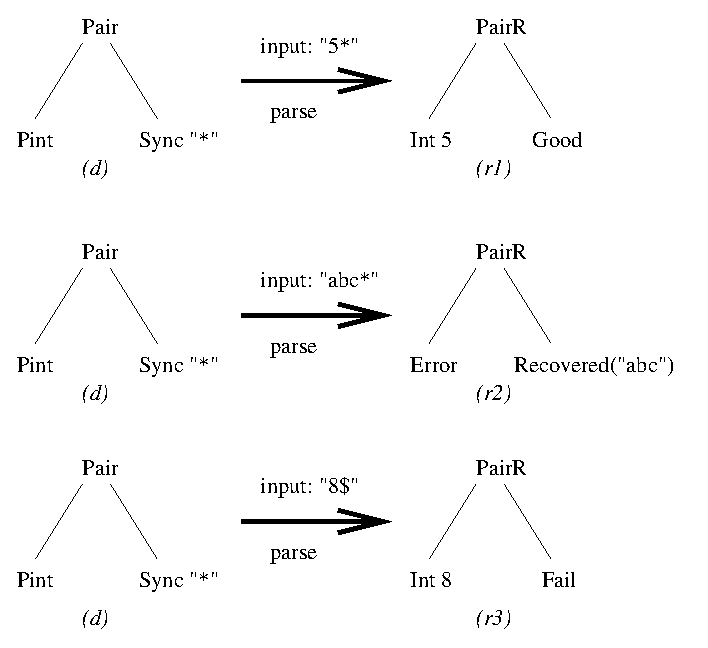
\includegraphics[width=0.8\columnwidth]{parse}
%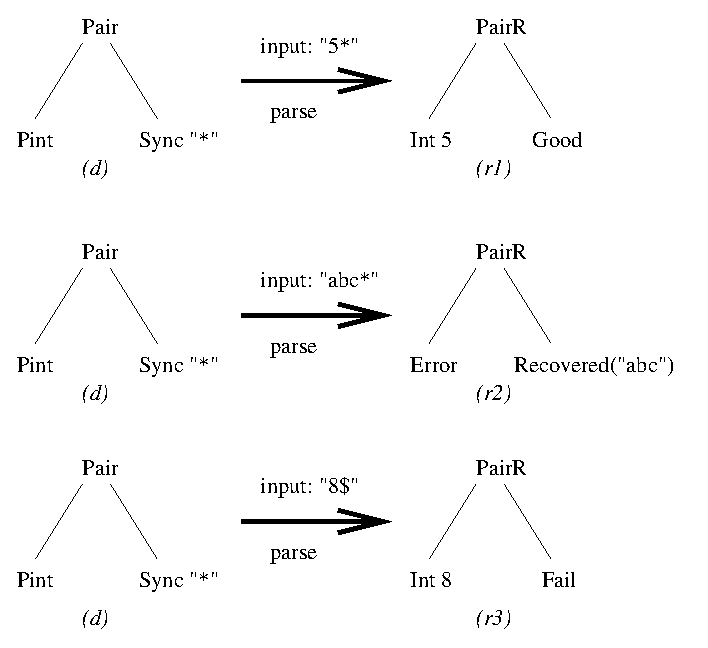
\epsfig{file=parse.eps, width=0.8\columnwidth}
\caption{Result of parsing three input lines}\label{fig:parse}
\end{center}
\end{figure}

\begin{figure*}[t]
\begin{center}
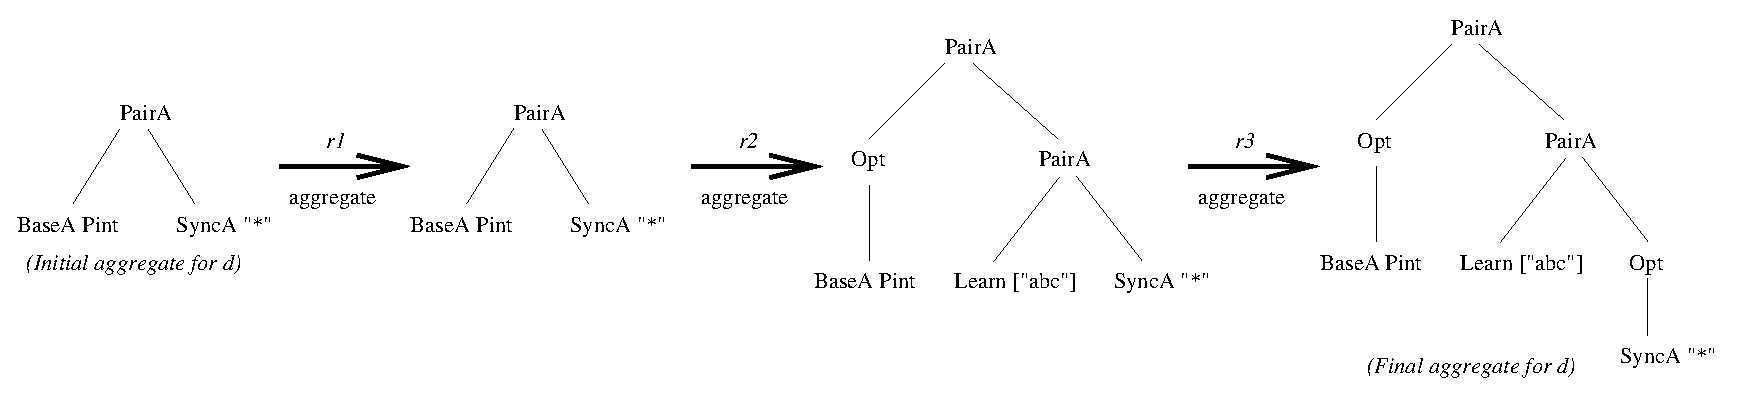
\includegraphics[width=2\columnwidth]{aggregate}
%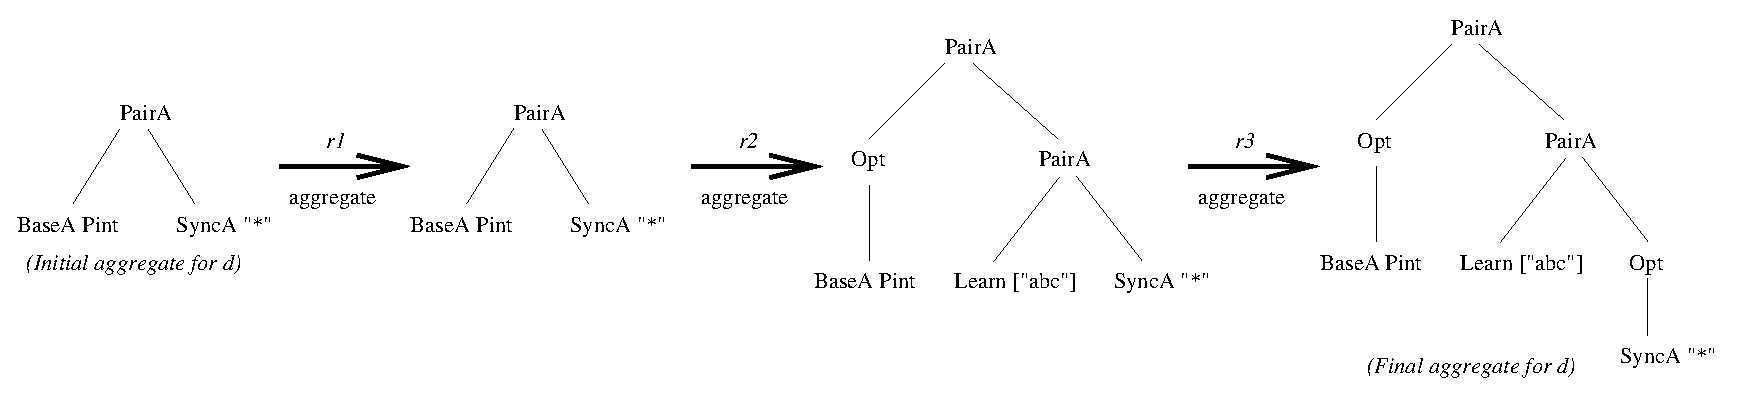
\epsfig{file=aggregate.eps, width=2\columnwidth}
\caption{Aggregation of three parses}\label{fig:aggregate}
\end{center}
\end{figure*}


%\begin{codebox}
%parse_all (d, x) =
%  switch (d) \{
%    case Pint =>  
%      (s, remainder) := match_prefix(x, "[0-9+\-]+");
%      if s != "" then return (Int s, remainder)
%      else return [(Error, x)];
%    case PstringME(re) => 
%      (s, remainder) := match_prefix(x, re);
%      if s != "" then return (Str s, remainder)
%      else return [(Error, x)];
%    case Sync s => 
%      (s', prefix, remainder) := match(x, s);
%      if s' = s and prefix = "" then return (Good, remainder)
%      elseif s' = "" then return (Fail, remainder)
%      else return [(Recovered prefix, remainder)]
%    case (x:d1, d2) =>
%      rs1 := parse_all (d1, x);
%      rs2 := [];
%      foreach (r1, remainder) in rs1 \{
%        (r2, remainder2) := parse_all (d2, remainder);
%        rs2 := rs2 + [((r1, r2), remainder2)]
%      \}
%    case (d1 + d2) => 
%	parse_all(d1, x) @ parse_all(d2, x)
%    case d array(sep, term) =>
%  \} 
%\end{codebox}    
%

\cut{%%%%%%%%%%%%%%%%%%%%%%%%%%%%%%%%

The {\tt parse\_all} function takes a description $d$ and an input string $x$, and returns
a list of all possible parses along with their respective ending position in the input. 
This function implements a standard recursive descent parser which recursively matches the
description structure (and sub-structures) with the input. To parse a pair $x: d_1 * d_2$, 
we first call {\tt parse\_all} on $d_1$ and get a list of parses. 
And then for each of the parse $r_1$ and corresponding end position, we bind $x$ to $r_1$ in
a private environment and  parse $d_2$ to get parses $l_2$. 
Finally for each parse $r_2$ in $l_2$ and each parse $r_1$ in $l_1$, 
construct a representation $(r_1, r_2)$, and return a list of all such pairs.
To parse a union $d_1 + d_2$, we simply return the concatenation of list of parses from
parsing $d_1$ and the list of parses from parsing $d_2$. To parse $d~ array(s, t)$,
we repeatedly attempt to parse $d$ until there's no more progress in the input.
And in each iteration, we also add parses generated from parsing $t$ as well, as if
the array has been terminated at this iteration. Figure \ref{fig:parse_base}
shows the {\tt parse\_base} function which parses a base token. The {\tt match\_prefix}
function matches the prefix of an input string with a regular expression and returns
the matched string and the remainder in the input. The {\tt match} function looks for
the first match of $s$ in input $x$, and returns the matched string $s'$, the prefix string
in $x$ before $s'$, and the remainder in the input.

\begin{figure}[t]
\begin{codebox}
parse_base (b, x) =
  switch (b) \{
  case Pint => 
    (s, suffix) := match_prefix(x, "[0-0+\-]+");
    if s <> "" then return [(Int s, suffix)];
    else return [(Error, x)]
  case PstringME(re) => 
    (s, suffix) := match_prefix(x, re);
    if s <> "" then return [(Str s, suffix)];
    else return [(Error, x)];
  case Sync s => 
    (s', prefix, remainder) := match(x, s);
    if s' = s and prefix = "" then 
      return (Good, remainder)
    elseif s' = "" then 
      return (Fail, remainder)
    else return [(Recovered prefix, remainder)]
  \}
\end{codebox}
\caption{Function to parse a base token or a sync token} \label{fig:parse_base}
\end{figure}

As an example, let $d$ be {\tt (Pint, Sync "|") + (PstringME "[a-z]+", Sync "|")}, 
and $x$ be ``\verb#abc|#''. {\tt parse\_all(d, x)} gives the following two possible parses:
{\small
\begin{verbatim}
  inl (Error, Recovered "abc")
  inr (Str "abc", Good)
\end{verbatim}
}

The {\tt aggregate} function adds a parse into an existing aggregate structure. When there is
no errors in the parse, it makes no changes to the aggregate. If the parse contains 
an error or failure for parsing token $b$, then the aggregate component 
$b$ is transformed to $opt~ b$, to indicate that $b$ node is optional. 
If a parse contains a recovered data $Recovered~ r$, then
a optional learn node will be created before the sync node. And the new aggregate component will be
$(opt (l [r]),~ Sync~ s)$. If the aggregate structure already contains the learn node before this
sync node, then recovered data $r$ will be added to the list under $l$.


}%%%%%%%%%%%%%%%%%%%%%%%%%%%%%%%%% END OF CUT %%%%%%%%%%%%%%%%

% - problem definition (as close to the previous description as possible) (but we don't
%   have a metric to measure how close yet, do we want to mention tree edit distance??)
% - overview of algorithm: parsing + aggregating + rewriting
% - parsing algo (parse rep, score metric, pseudo-code)
% - aggregating algo (in pseudo code)
% - selection of top aggregates
% - update original description
% - rewriting rules (data independent, data dependent, OptsTable)


\subsection{Description Rewriting}
Once we have successfully parsed, aggregated and relearned a new
chunk of data, we optimize the new description using rewriting rules.  
Our original non-incremental
algorithm already had such an optimization
phase; we have modified and tuned the algorithm for use in
the incremental system.

Description rewriting is based on optimizing an information-theoretic
Minimum Description Length (MDL) score~\cite{mdlbook}, which is 
defined over descriptions
\cd{D} as:
\[\mbox{\rm{MDL}(\texttt{D})} = \costdescription{D} + w \times \acostdata{D}{x_1, \ldots, x_k},\]
where $\costdescription{D}$ is called the {\em type complexity} of \cd{D}
and \\
$\acostdata{D}{x_1, \ldots, x_k}$ is called the {\em atomic data 
complexity}.  The type complexity is a measure of the size of the 
abstract syntax of \cd{D}.  The atomic data 
complexity of data records $x_1, \ldots, x_k$ relative to \cd{D} 
is the number of bits required
to transmit an {\em average} data record given the description \cd{D}.
The MDL score of \cd{D} is the weighted sum of these two components.  
Our experiments indicate a weight $w$ of approximately 10 is effective
in our domain.

Given a rewriting rule that rewrites \cd{D} to \cd{D'}, the
rule fires if and only if \rm{MDL}(\texttt{D}) $\leq$ \rm{MDL}(\texttt{D'}).
Rewriting continues until no further rule can fire.
Hence, our rewriting strategy is a greedy local
search.

\begin{figure}[t]
\begin{center}
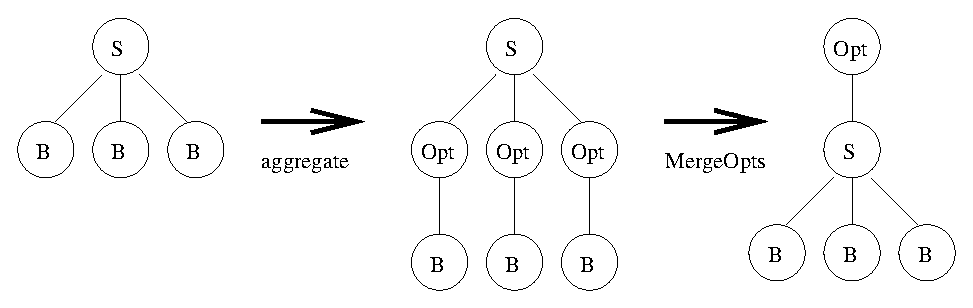
\includegraphics[width=\columnwidth]{opts}
%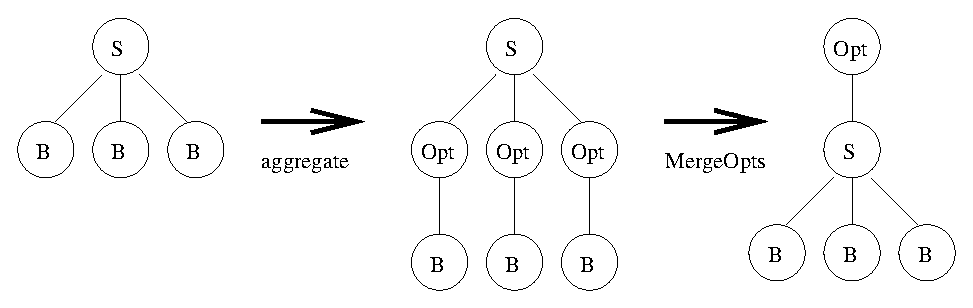
\epsfig{file=opts.eps,width=\columnwidth}
\caption{MergeOpts rewriting rule}\label{fig:opts}
\end{center}
\vskip -2ex
\end{figure}

%% When the incremental learning algorithm produces a refined description
%% from an aggregate, the algorithm applies rewriting rules
%% to the new description to improve its quality and readability.
%% Most of the rules are data-independent and inherited from \learnpads{}, such as 
%% removing degenerate lists and flattening nested structs and unions.

The original learning system contains many MDL-based rewriting rules, for example,
to flatten nested structs and unions and
to refine ranged types.
{\em BlobFinding} is an important new rewriting rule. 
This rule takes a given sub-description \cd{D} and uses a heuristic to 
determine if the type complexity of \cd{D} is too high relative to the amount of data it covers.
The heuristic is that if the height of \cd{D} is larger than \cd{minBlobHeight}
(which is empirically determined to be 4 in this paper), and there is an identifiable constant string 
or pattern \cd{re} that immediately follows
\cd{D}, then we rewrite \cd{D} to 
\cd{Pstring\_SE(:re:)}.
Description \cd{Pstring\_SE} is a \pads{} base type that is similar to \cd{Pstring},
except it uses a stopping regular pattern as opposed to a stopping character
to indicate termination. This rule is tremendously helpful
in controlling the size and
complexity of learned descriptions.  Without it, descriptions can
grow in complexity to the point where parsing is slow and the algorithm fails to scale.


We also introduced a new {\em data dependent} rewriting rule called {\em MergeOpts}
to optimize a pattern that occurs frequently in descriptions during incremental
learning.  Recall that the aggregate function
introduces \cd{Opt} nodes above a \cd{BaseA} or \cd{SyncA} node 
whenever the corresponding \cd{Base} or \cd{Sync} token in 
the description failed to 
parse. When faced with an entirely new form of data, 
the algorithm is likely to introduce a series of \cd{Opt} nodes as
each type in the original description fails in succession. 
The {\em MergeOpts} rule collapses these consecutive \cd{Opt} nodes if they
are correlated, \ie{}, either they are all always present or all always
absent.  To verify this correlation, the algorithm maintains a
table that records the branching decisions when parsing each
data line. It uses this table to determine whether to merge
adjacent \cd{Opt} nodes during rewriting. 
\figref{fig:opts} illustrates the effect of this rule.  In the figure,
$S$ denotes a struct and $B$ a base token.

\vspace{20pt}


\section{Implementation}\label{sec:imp}

For purposes of presentation, we have described an idealized and
unoptimized algorithm.  Our actual implementation includes a number of
refinements to improve the quality of the description and/or reduce the
inference time.  In this section, we discuss some of these refinements.

\subsection{Token families}
So far, parsing a \cd{Sync} token yields
one of three results: \cd{Good}, \cd{Fail} or \cd{Recovered}. 
In the actual implementation, a \cd{Sync} token can be not only a constant string, but also
a constant integer, an integer range or a combination thereof.
Consider parsing the token \cd{Sync (Str "GET")} when
the current input starts with ``POST.'' The
\cd{parse\_base} function indicates the result should be \cd{Fail}.
In reality, the input ``POST'' is in the same {\em family} as ``GET,'' 
\ie{}, a word,
and it may very well be that this \cd{Sync} token should have been 
an enumeration of words rather than a single word.
To handle such cases, we created a fourth type of parse node, \cd{Partial}, 
to indicate that the input belongs to the same family as the expected
token but does not match exactly, \ie, it is {\em partially} correct.
During aggregation, partial nodes cause the description 
to be specialized to include the additional values.  In the above example, the aggregate 
function will change the description to \cd{Sync (Enum [Word "GET", Word "POST"])}.
Such partial nodes reduce the number of parsing errors
and produce more compact and meaningful descriptions.


\subsection{Rewriting rules}
When the incremental learning algorithm produces a refined description
from an aggregate, the algorithm applies rewriting rules
to the new description to improve its quality and readability.
Most of the rules are data-independent and inherited from \learnpads{}, such as 
removing degenerate lists and flattening nested structs and unions.
We introduce one new {\em data dependent} rule called {\em MergeOpts}
to optimize a type pattern that occurs frequently during incremental
learning.  Recall that the aggregate function
introduces \cd{Opt} nodes above a \cd{BaseA} or \cd{SyncA} node 
whenever the corresponding \cd{Base} or \cd{Sync} token in the description failed to 
parse. When faced with an entirely new form of data, 
the algorithm is likely to introduce a series of \cd{Opt} nodes as
each type in the original description fails in succession. 
The {\em MergeOpts} rule collapses these consecutive \cd{Opt} nodes if they
are correlated, \ie{}, either they are all always present or all always
absent.  To verify this correlation, the algorithm maintains a
table that records the branching decisions when parsing each
data line. It uses this table to determine whether to merge
adjacent \cd{Opt} nodes during rewriting. 
\figref{fig:opts} illustrates the effect of this rule.  In the figure,
$S$ denotes a struct and $B$ a base token.

\begin{figure}[t]
\begin{center}
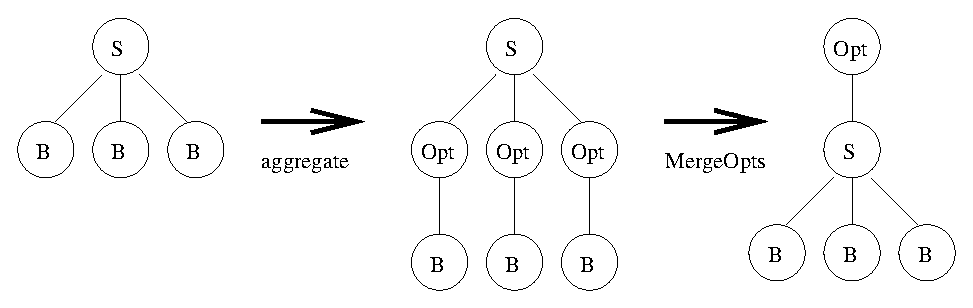
\includegraphics{opts}
%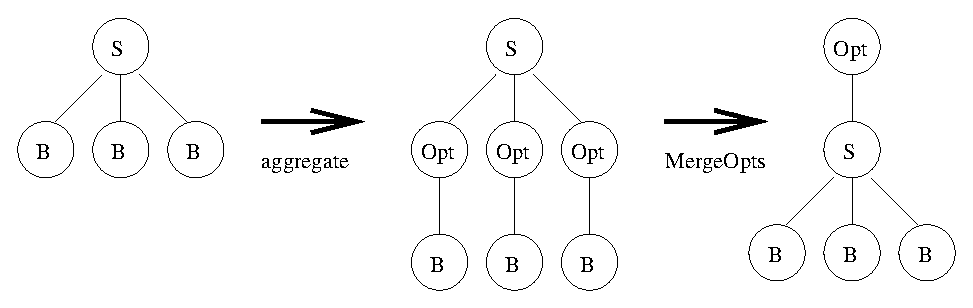
\epsfig{file=opts.eps,width=\columnwidth}
\caption{MergeOpts rewriting rule}\label{fig:opts}
\end{center}
\vskip -2ex
\end{figure}


\subsection{Performance}
The pseudo-code in \figref{fig:inc-learning} suggests the number of
aggregates is of the order $O(m ^ n)$, where $m$ is the maximum number of
parses for a line of input  and $n$ is the number of lines to
aggregate.  Clearly, this algorithm will not scale 
unless $m$ and $n$ are bounded.

We have implemented several optimizations to limit the number of 
parses and aggregates. First, we do not return all possible
parses when parsing a description component \cd{D}. 
Instead, we rank the parses by a metric that
measures their quality and return only the top $k$. The metric is
a triple: 
$m = (e,~ s,~ c)$,
where $e$ is the number of errors, $s$ is the number of 
characters skipped during \cd{Sync} token recovery, and $c$ is the number
of characters correctly parsed. The metric is considered \textit{perfect} if $e = 0$.
Metric $m_1$ is better than $m_2$ if $m_1$ is perfect and $m_2$ is not, or
if 
\[\frac{c_1}{s_1+c_1} > \frac{c_2}{s_2 + c_2}.\]

In practice, \cd{parse} returns a list of
{\em parse triples} $(r,~m,~j)$, where $r$ is the data representation of
the parse, $m$ is the metric associated with $r$, and
$j$ is the position in the input after the parse.
We define a \cd{clean} function that first partitions the
triples into groups that share the same 
{\em span}, \ie{}, the substring of the input consumed by the parse.
For each group, \cd{clean} retains all perfect parses. If 
none exists, it retains the best parse in the group. 
We justify discarding the other triples because
given a description $d$ and a fixed span, we always
prefer the parse with the best metric. This idea is
similar to the dynamic programming techniques used in 
Earley Parsers \cite{earley-parser}. Finally \cd{clean} returns all
the perfect triples plus up to the top $k$ non-perfect triples.
The \cd{clean} function reduces the number of bad parses 
to a constant $k$ while guaranteeing that if there is a
perfect parse, it will be returned. 

A second optimization, which we call {\em parse cut-off}, terminates a
candidate parse when parsing a struct with multiple
fields $f_1$, $f_2$, ..., $f_n$ if the algorithm encounters 
a threshold number of errors in succession. 
This technique may result in no possible parses for the
top-level description.  In this case, we restart the process
with the parse cut-off optimization turned off. 
A third optimization is memoization.
The program keeps a global memo table indexed by the pair of a
description \cd{D} and the beginning position for parsing \cd{D} which
stores the result for parsing \cd{D} at the specific position.
Finally, we bound the total number of aggregates the
algorithm can produce by selecting the top
$k$ aggregates with the fewest number of \cd{Opt} and \cd{Learn}
nodes. 



\section{Evaluation}
\label{sec:eval}
The following experiments were done on a PowerBook G4 with a 1.67GHz PowerPC
CPU and 2G memory running on Mac OS X 10.4. 
Table \ref{tab:results} compares the performance results between
the original \learnpads{} system and the incremental system. 
The benchmarks used are 12 system logs with various sizes. Column 2
shows the number of lines in each log. The time columns record the total
running time in seconds, and the TC columns record the type complexity
of the final description learned. In general, lower type complexity means
more compact description. For the first 7 benchmarks which are smaller
and simpler, the initial learn size is 100 lines and the 
incremental learn size is 100 lines. For the last 5 benchmarks, 
the initial learn size is 500 lines while the incremental size remains
100 lines. Where it takes more than half an hour for the original \learnpads{}
system to learn a description, a ``-'' is put in those cells to 
indicate there is no result.

\begin{table}[th]
\begin{tabular}{|c|c|c|c|c|c|}\hline
& & \multicolumn{2}{|c|}{original} & \multicolumn{2}{|c|}{incremental} \\ \cline{3-6}
\raisebox{1.5ex}[0pt]{Formats} & \raisebox{1.5ex}[0pt]{Lines} &
	Time & TC & Time & TC \\ \hline \hline
ai.3000	&	3000	& 32	& 412.6	& 2.2	& 571.0	\\ \hline
asl.log  &	1500	& 31.9	& 960.1	& 23.9 	& 1393.3 \\ \hline
apache.txt  &	2087	& 83.9 & 1746.1 & 7.9 	& 2527.6 \\ \hline
access\_log  &	8188 	& 134.5	& 351.2	& 2.9	& 321.2	\\ \hline
error\_log  &	4510	& 101.7	& 101.9	& 0.9	& 107.9 \\ \hline
interface.loop & 1253	& 54.0	& 741.4	& 1.9	& 1053.7 \\ \hline
ai.big	&	57368	& -	& -	& 30	& 533.9 \\ \hline
pws	&	 17365	& -	& - 	& 133  & 5869 \\ \hline
coblitz.access & 9421   & -	& -	& 31.9 & 3005.2 \\ \hline
access.exlog & 260796 	& -	& -	& 610 & 3088.3 \\ \hline
debug\_getbig & 550409   & -	& -	& 668 & 9008.1 \\ \hline
dbg\_req\_redirect & 302554 & -	& -	& 1852 & 17567.7 \\ \hline
\end{tabular}
\caption{Execution times (secs) and type complexity (bits)} 
\label{tab:results}
\end{table}


% - parse metric
% - initial learn size and chunk size - these can affect results
% - update chunk by chunk 
% - optimizations/heuristics
%   due to performance concerns:
%   - memoization
%   - the clean function (to reduce the number of parses)
%   - control of aggregate size
%   - parses cut-off: kill a parse if it has more than n consecutive failures in a struct
%   due to quality of description concerns (and also performance)
%   - deterministic unions
%   - longest match in arrays
%   - merge adjacent const strings (only punctuation and white spaces)
%   - error recovery
%
%- Experiments
%	1) comparison with old LearnPADS on several large datasets (ai.3000, asl.log, apache.txt, access\_log, error\_log, interface.loop)
%	   compare exec time and type complexity. For increment, use
%	   initial learn chunk of 100 and incremental error chunks of 100
%	2) use ai format, do a table with 1000 5000 10000,...,1M miles
%	   using orig learning system and the new system with various optimization turned on and off.
%



The explosive growth of the internet has made monitoring and managing
data systems distributed across wide-area networks increasingly
important.  The possibility of partial failure and the need to
synchronize makes such code tedious and difficult to write correctly,
particularly for data experts whose skills are in domains other than
networking. In this paper, we describe the \padsd{} system, which
allows users to declaratively specify their data systems and then
generate a wide-variety of tools for manipulating the data: from
stand-alone tools, to simple libraries for writing their own analyses,
to generic libraries for building new generic tools.  We precisely
specify the meaning of our language via a sound denotational
semantics and show via experimentation that the system has
acceptable performance overheads.


\section*{Acknowledgments}
This material is based upon work
 supported by the NSF under grants 0612147 and 0615062, and
a gift from Google. Any opinions, findings, and conclusions or recommendations
expressed in this material are those of the authors and do not
necessarily reflect the views of the NSF or Google.

\bibliographystyle{plain}
%\bibliographystyle{abbrv}

\bibliography{pads}

%%\newpage
\appendix

\section{Example Data and Descriptions}
\label{app:examples}


%%% Local Variables: 
%%% mode: latex
%%% TeX-master: "semantics"
%%% End: 


\end{document}

%%% Local Variables:
%%% mode: outline-minor
%%% End:

